\documentclass{article}
%\usepackage{pgf}
%\usepackage{tikz}
%\usetikzlibrary{arrows,automata}
%%\usepackage[latin1]{inputenc}
\usepackage{tikz}
\usepackage{pgfplots}
\usepackage{graphicx}
\usepackage{caption}
\usepackage{subcaption}

%\usepackage{pgfplots}
%\usepackage{pgfplotstable}
%	\pgfplotsset{compat=newest}
%	\newlength\figureheight
%	\newlength\figurewidth
%\usepackage{tikz}
%	\usetikzlibrary{external, backgrounds, patterns, shapes, shapes.multipart,positioning,arrows.meta,arrows,calc,arrows,decorations.pathmorphing}
%	\tikzexternalize[shell escape=-enable-write18,prefix=tikz/]
%	\tikzexternaldisable

\begin{document}
test

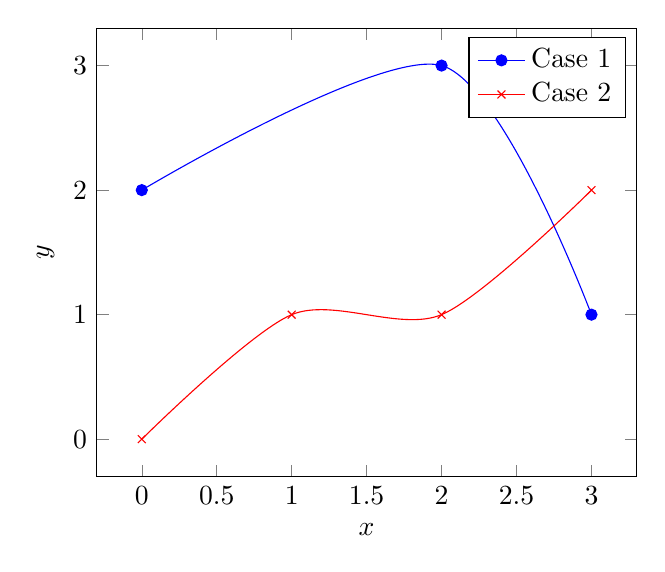
\begin{tikzpicture}
    \begin{axis}[
        xlabel=$x$,
        ylabel=$y$]
    \addplot[smooth,mark=*,blue] plot coordinates {
        (0,2)
        (2,3)
        (3,1)
    };
    \addlegendentry{Case 1}

    \addplot[smooth,color=red,mark=x]
        plot coordinates {
            (0,0)
            (1,1)
            (2,1)
            (3,2)
        };
    \addlegendentry{Case 2}
    \end{axis}
    \end{tikzpicture}

\begin{figure}
\begin{subfigure}[b]{0.54\linewidth}
\scalebox{0.5}{
% This file was created by matlab2tikz.
%
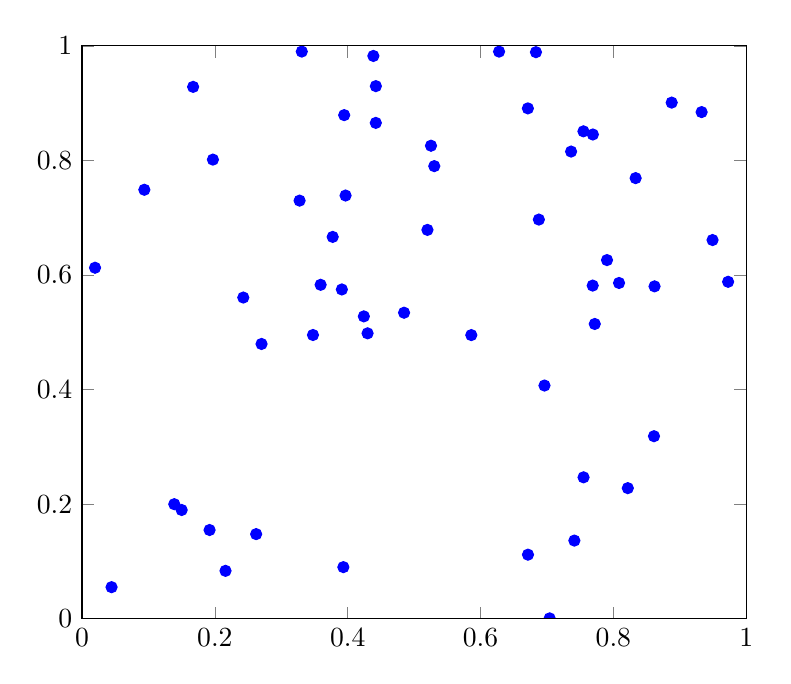
\begin{tikzpicture}
\begin{axis}[%
%width=\figurewidth,
%height=\figureheight,
scale only axis,
xmin=0,
xmax=1,
ymin=0,
ymax=1,
%every tick label/.append style={font=\tiny},
axis background/.style={fill=white},
clip marker paths=true, axis on top=true]
\addplot [color=blue,only marks,mark=*,mark options={solid,fill=blue},forget plot]
  table[row sep=crcr]
  {
0.627896379614169	0.989872153631504 \\
0.771980385554245	0.514423456505704\\
0.93285357027882	0.884281023126955\\
0.972740854003014	0.588026055308497\\
0.192028349427775	0.154752348656045\\
0.138874202829155	0.199862822857452\\
0.696266337082995	0.406954837138907\\
0.0938200267748656	0.748705718215691\\
0.525404403859336	0.825583815786156\\
0.530344218392863	0.789963029944531\\
0.861139811393332	0.318524245398992\\
0.484853333552102	0.534064127370726\\
0.393456361215266	0.089950678770581\\
0.671431139674026	0.111705744193203\\
0.741257943454206	0.136292548938299\\
0.520052467390387	0.678652304800188\\
0.347712671277525	0.495177019089661\\
0.149997253831683	0.18971040601758\\
0.586092067231462	0.495005824990221\\
0.262145317727807	0.147608221976689\\
0.0444540922782385	0.0549741469061882\\
0.754933267231179	0.850712674289007\\
0.242785357820962	0.560559527354885\\
0.442402313001943	0.929608866756663\\
0.687796085120107	0.696667200555228\\
0.359228210401861	0.58279096517584\\
0.736340074301202	0.815397211477421\\
0.394707475278763	0.879013904597178\\
0.683415866967978	0.988911616079589\\
0.704047430334266	0.000522375356944771\\
0.442305413383371	0.865438591013025\\
0.0195776235533187	0.612566469483999\\
0.330857880214071	0.989950205708831\\
0.424309496833137	0.527680069338442\\
0.270270423432065	0.479523385210219\\
0.197053798095456	0.801347605521952\\
0.82172118496131	0.227842935706042\\
0.429921409383266	0.49809429119639\\
0.887770954256354	0.900852488532005\\
0.391182995461163	0.574661219130188\\
0.769114387388296	0.845178185054037\\
0.396791517013617	0.738640291995402\\
0.808514095887345	0.585987035826476\\
0.755077099007084	0.246734525985975\\
0.377395544835103	0.666416217319468\\
0.216018915961394	0.0834828136026227\\
0.790407217966913	0.625959785171583\\
0.949303911849797	0.660944557947342\\
0.327565434075205	0.729751855317221\\
0.67126437045174	0.890752116325322\\
0.438644982586956	0.982303222883606\\
0.833500595588975	0.769029085335896\\
0.768854252429615	0.581446487875398\\
0.167253545494722	0.928313062314188\\
0.861980478702072	0.580090365758442\\
};
\end{axis}
\end{tikzpicture}%
}
\end{subfigure}
\begin{subfigure}[b]{0.45\linewidth}
\scalebox{0.5}{
% This file was created by matlab2tikz.
%
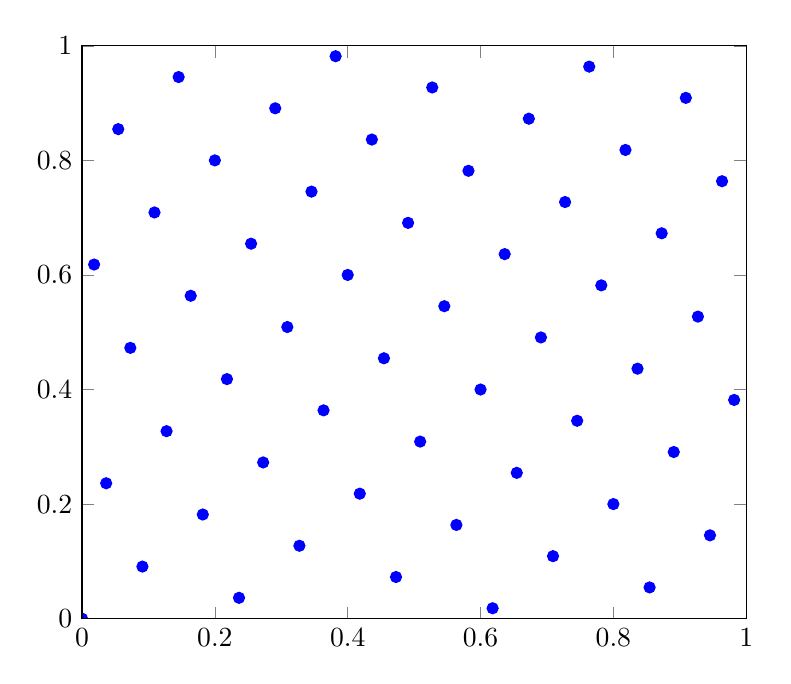
\begin{tikzpicture}


\begin{axis}[%
%width=\figurewidth,
%height=\figureheight,
scale only axis,
xmin=0,
xmax=1,
ymin=0,
ymax=1,
%every tick label/.append style={font=\tiny},
axis background/.style={fill=white},
clip marker paths=true, axis on top=true
]
\addplot [color=blue,only marks,mark=*,mark options={solid,fill=blue},forget plot]
  table[row sep=crcr]
  {%
0	0\\
0.0181818181818182	0.618181818181818\\
0.0363636363636364	0.236363636363636\\
0.0545454545454545	0.854545454545454\\
0.0727272727272727	0.472727272727273\\
0.0909090909090909	0.0909090909090908\\
0.109090909090909	0.709090909090909\\
0.127272727272727	0.327272727272727\\
0.145454545454545	0.945454545454545\\
0.163636363636364	0.563636363636363\\
0.181818181818182	0.181818181818182\\
0.2	0.8\\
0.218181818181818	0.418181818181818\\
0.236363636363636	0.036363636363637\\
0.254545454545455	0.654545454545454\\
0.272727272727273	0.272727272727273\\
0.290909090909091	0.890909090909091\\
0.309090909090909	0.50909090909091\\
0.327272727272727	0.127272727272727\\
0.345454545454545	0.745454545454546\\
0.363636363636364	0.363636363636363\\
0.381818181818182	0.981818181818182\\
0.4	0.6 \\
0.418181818181818	0.218181818181819\\
0.436363636363636	0.836363636363636\\
0.454545454545455	0.454545454545455\\
0.472727272727273	0.0727272727272741\\
0.490909090909091	0.690909090909091\\
0.509090909090909	0.309090909090909\\
0.527272727272727	0.927272727272726\\
0.545454545454545	0.545454545454547\\
0.563636363636364	0.163636363636364\\
0.581818181818182	0.781818181818181\\
0.6	0.399999999999999\\
0.618181818181818	0.0181818181818194\\
0.636363636363636	0.636363636363637\\
0.654545454545455	0.254545454545454\\
0.672727272727273	0.872727272727271\\
0.690909090909091	0.490909090909092\\
0.709090909090909	0.109090909090909\\
0.727272727272727	0.727272727272727\\
0.745454545454545	0.345454545454544\\
0.763636363636364	0.963636363636365\\
0.781818181818182	0.581818181818182\\
0.8	0.199999999999999\\
0.818181818181818	0.818181818181817\\
0.836363636363636	0.436363636363637\\
0.854545454545454	0.0545454545454547\\
0.872727272727273	0.672727272727272\\
0.890909090909091	0.290909090909089\\
0.909090909090909	0.90909090909091\\
0.927272727272727	0.527272727272727\\
0.945454545454545	0.145454545454548\\
0.963636363636364	0.763636363636365\\
0.981818181818182	0.381818181818183\\
};
\end{axis}
\end{tikzpicture}%}
\end{subfigure}
\end{figure}

%\begin{tikzpicture}[->,>=stealth',shorten >=1pt,auto,node distance=2.8cm,
%                    semithick]
%  \tikzstyle{every state}=[fill=red,draw=none,text=white]
%
%  \node[initial,state] (A)                    {$q_a$};
%  \node[state]         (B) [above right of=A] {$q_b$};
%  \node[state]         (D) [below right of=A] {$q_d$};
%  \node[state]         (C) [below right of=B] {$q_c$};
%  \node[state]         (E) [below of=D]       {$q_e$};
%
%  \path (A) edge              node {0,1,L} (B)
%            edge              node {1,1,R} (C)
%        (B) edge [loop above] node {1,1,L} (B)
%            edge              node {0,1,L} (C)
%        (C) edge              node {0,1,L} (D)
%            edge [bend left]  node {1,0,R} (E)
%        (D) edge [loop below] node {1,1,R} (D)
%            edge              node {0,1,R} (A)
%        (E) edge [bend left]  node {1,0,R} (A);
%\end{tikzpicture}


%\begin{figure}
%% This file was created by matlab2tikz.
%
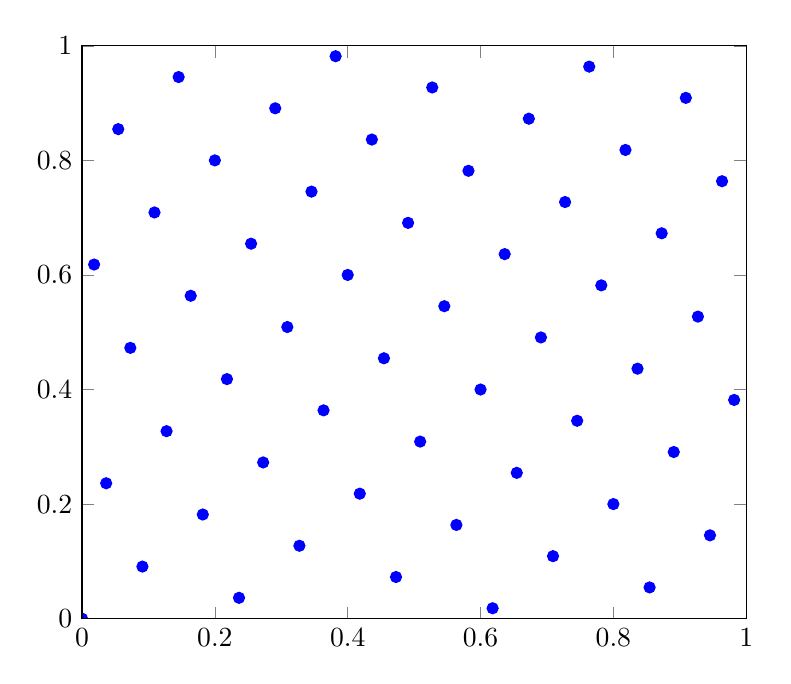
\begin{tikzpicture}


\begin{axis}[%
%width=\figurewidth,
%height=\figureheight,
scale only axis,
xmin=0,
xmax=1,
ymin=0,
ymax=1,
%every tick label/.append style={font=\tiny},
axis background/.style={fill=white},
clip marker paths=true, axis on top=true
]
\addplot [color=blue,only marks,mark=*,mark options={solid,fill=blue},forget plot]
  table[row sep=crcr]
  {%
0	0\\
0.0181818181818182	0.618181818181818\\
0.0363636363636364	0.236363636363636\\
0.0545454545454545	0.854545454545454\\
0.0727272727272727	0.472727272727273\\
0.0909090909090909	0.0909090909090908\\
0.109090909090909	0.709090909090909\\
0.127272727272727	0.327272727272727\\
0.145454545454545	0.945454545454545\\
0.163636363636364	0.563636363636363\\
0.181818181818182	0.181818181818182\\
0.2	0.8\\
0.218181818181818	0.418181818181818\\
0.236363636363636	0.036363636363637\\
0.254545454545455	0.654545454545454\\
0.272727272727273	0.272727272727273\\
0.290909090909091	0.890909090909091\\
0.309090909090909	0.50909090909091\\
0.327272727272727	0.127272727272727\\
0.345454545454545	0.745454545454546\\
0.363636363636364	0.363636363636363\\
0.381818181818182	0.981818181818182\\
0.4	0.6 \\
0.418181818181818	0.218181818181819\\
0.436363636363636	0.836363636363636\\
0.454545454545455	0.454545454545455\\
0.472727272727273	0.0727272727272741\\
0.490909090909091	0.690909090909091\\
0.509090909090909	0.309090909090909\\
0.527272727272727	0.927272727272726\\
0.545454545454545	0.545454545454547\\
0.563636363636364	0.163636363636364\\
0.581818181818182	0.781818181818181\\
0.6	0.399999999999999\\
0.618181818181818	0.0181818181818194\\
0.636363636363636	0.636363636363637\\
0.654545454545455	0.254545454545454\\
0.672727272727273	0.872727272727271\\
0.690909090909091	0.490909090909092\\
0.709090909090909	0.109090909090909\\
0.727272727272727	0.727272727272727\\
0.745454545454545	0.345454545454544\\
0.763636363636364	0.963636363636365\\
0.781818181818182	0.581818181818182\\
0.8	0.199999999999999\\
0.818181818181818	0.818181818181817\\
0.836363636363636	0.436363636363637\\
0.854545454545454	0.0545454545454547\\
0.872727272727273	0.672727272727272\\
0.890909090909091	0.290909090909089\\
0.909090909090909	0.90909090909091\\
0.927272727272727	0.527272727272727\\
0.945454545454545	0.145454545454548\\
0.963636363636364	0.763636363636365\\
0.981818181818182	0.381818181818183\\
};
\end{axis}
\end{tikzpicture}%
%\end{figure}
\end{document}
